%\documentclass[mathserif]{beamer}
\documentclass[handout]{beamer}
%\usetheme{Goettingen}
\usetheme{Warsaw}
%\usetheme{Singapore}
%\usetheme{Frankfurt}
%\usetheme{Copenhagen}
%\usetheme{Szeged}
%\usetheme{Montpellier}
%\usetheme{CambridgeUS}
%\usecolortheme{}
%\setbeamercovered{transparent}
\usepackage[utf8x]{inputenc} 
\usepackage[spanish]{babel} %idioma
\usepackage{amsmath, amssymb}
\usepackage{dsfont}
\usepackage{graphics}
\usepackage{cases}
\usepackage{graphicx}
\usepackage{pgf}
\usepackage{epsfig}
\usepackage{amssymb}
\usepackage{amstext}
\usepackage[ruled,vlined,lined]{algorithm2e}
\usepackage{amsmath}
\usepackage{epic}
\usepackage{epsfig}
\usepackage{fontenc}
\usepackage{palatino, url, multicol}
%\algsetup{indent=2em}
\newcommand{\factorial}{\ensuremath{\mbox{\sc Factorial}}}
\newcommand{\BIGOP}[1]{\mathop{\mathchoice%
{\raise-0.22em\hbox{\huge $#1$}}%
{\raise-0.05em\hbox{\Large $#1$}}{\hbox{\large $#1$}}{#1}}}
\newcommand{\bigtimes}{\BIGOP{\times}}
\vspace{-0.5cm}
\title{Modelos Lineales y Redes Neuronales}
\vspace{-0.5cm}
\author[Felipe Bravo Márquez]{\footnotesize
%\author{\footnotesize  
 \textcolor[rgb]{0.00,0.00,1.00}{Felipe José Bravo Márquez}} 

%\vspace{-0.3cm}
\institute{Universidad de Chile- Minería de Datos}
\date{ \today }


\begin{document}
\begin{frame}
\titlepage


\end{frame}


%%%%%%%%%%%%%%%%%%%%%%%%%%%



\begin{frame}{Modelos de Regresión}
\scriptsize{
\begin{itemize}

 \item Un modelo de regresión se usa para modelar la relación de una variable dependiente $\mathbf{y}$ numérica con $n$ variables independientes $\mathbf{x}_1, \mathbf{x}_2, \dots, \mathbf{x}_n$. 
 
 \item A grandes rasgos queremos conocer el valor esperado de $\mathbf{y}$ a partir los valores de $\mathbf{x}$:
 \begin{displaymath}
 \mathbb{E}(y|x_1,x_2,\dots,x_n)
 \end{displaymath}

 
 \item Usamos estos modelos cuando creemos que la variable de respuesta $\mathbf{y}$ puede ser modelada por otras variables independientes también conocidas como covariables o atributos.
 
 \item Para realizar este tipo de análisis necesitamos un dataset formado por $m$ observaciones que incluyan tanto a la variable de respuesta como a cada uno de los atributos.
 
 \item Nos referimos al proceso de \textbf{ajustar} una función de regresión al proceso en que a partir de los datos inferimos una función de hipótesis $h$ que nos permite predecir valores de $\mathbf{y}$ desconocidos usando los valores de los atributos.

 
\end{itemize}



} 
 
\end{frame}


\begin{frame}{Introducción (2)}
\scriptsize{
\begin{itemize}
 
 \item A este proceso de ajustar una función a partir de los datos se le llama en las áreas de minería de datos y aprendizaje de máquinas como \textbf{entrenamiento}.

 \item En esas disciplinas se dice que las funciones \textbf{aprenden} a partir de los datos.
 
 \item Como necesitamos observaciones donde el valor de $\mathbf{y}$ sea conocido para aprender la función,  se le llama a este tipo de técnicas como técnicas de \textbf{aprendizaje supervisado}.
 
 \item Cuando $\mathbf{y}$ es una variable categórica hablamos de un problema de \textbf{clasificación}.
 

 
\end{itemize}


\begin{figure}[h!]
	\centering
	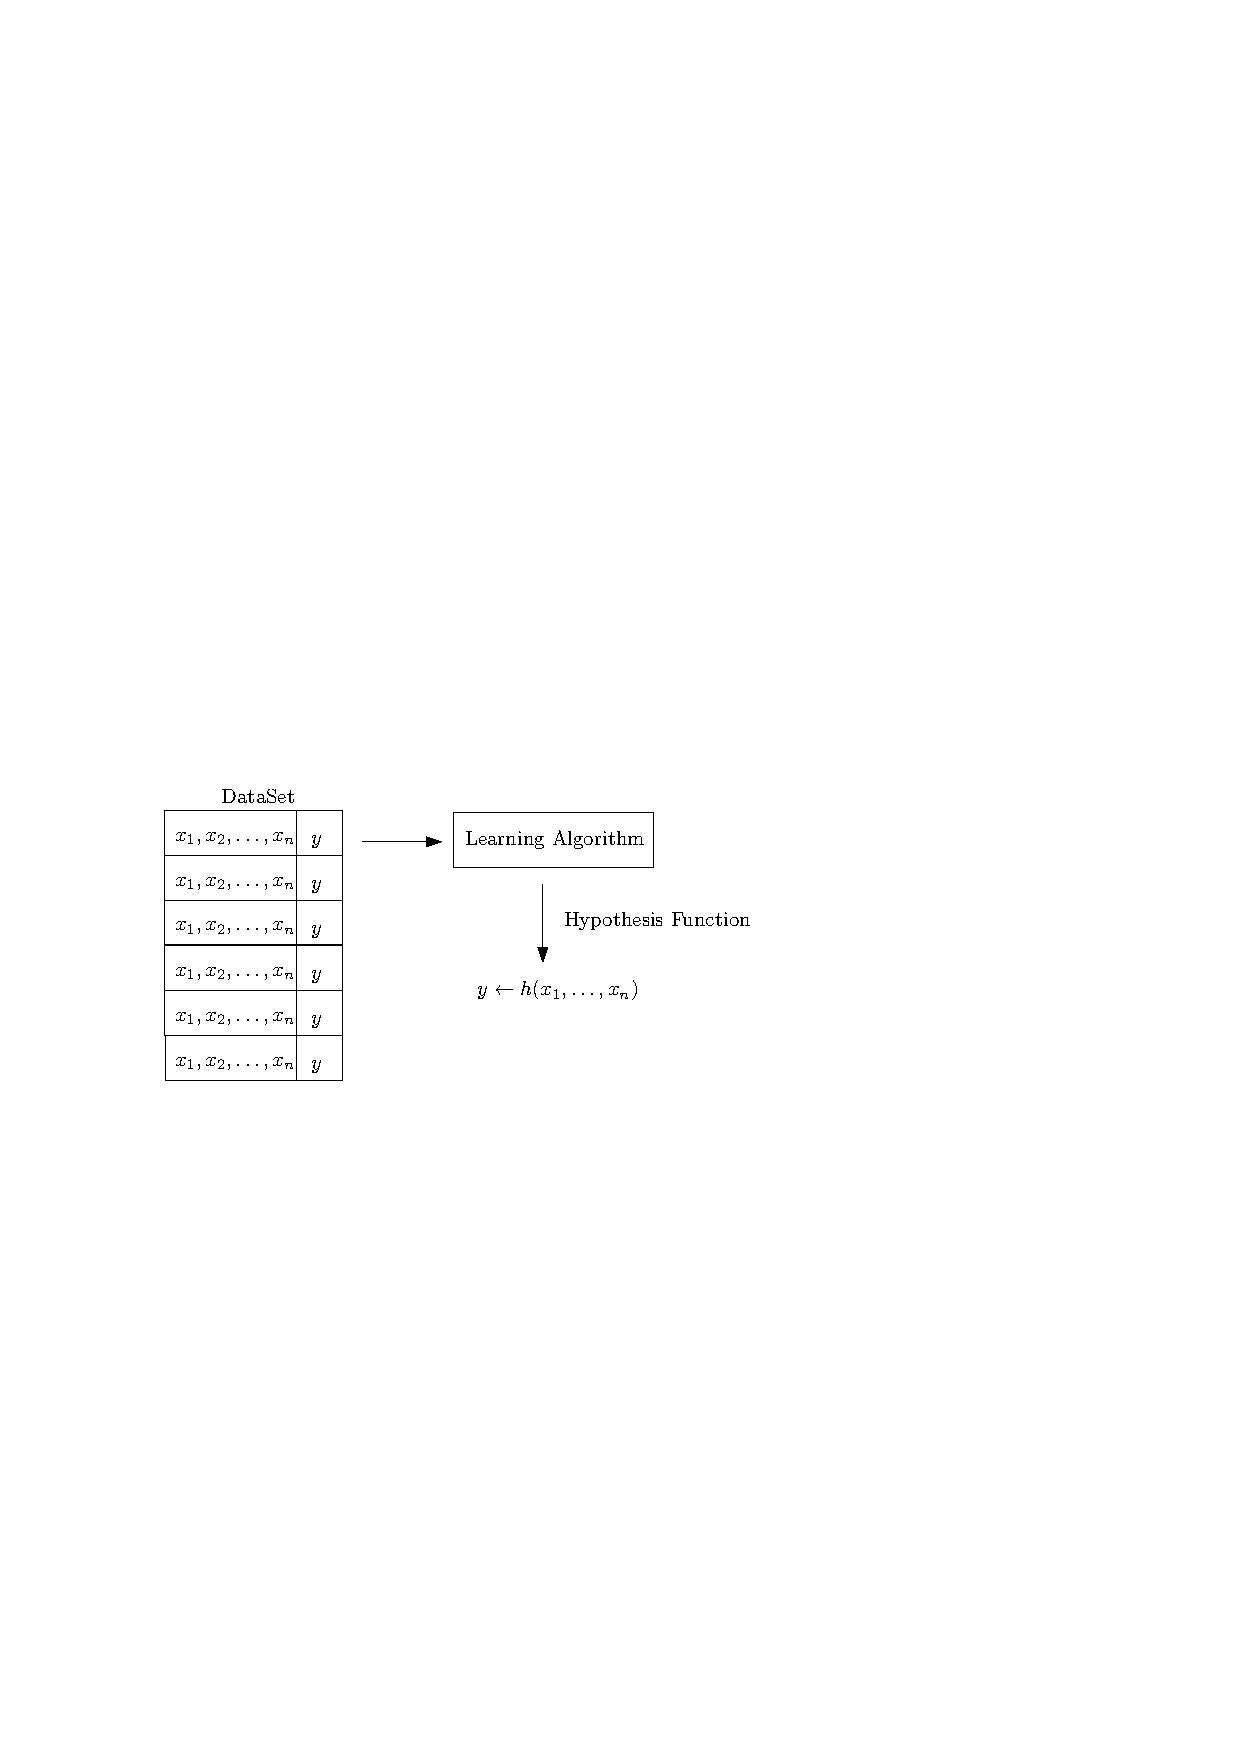
\includegraphics[scale=0.65]{imagenes/learning.pdf}
\end{figure}

} 
 
\end{frame}


\begin{frame}{Regresión Lineal Simple}
\scriptsize{
\begin{itemize}
 \item En la regresión lineal simple se tiene una única variable independiente $x$ para modelar la variable dependiente $\mathbf{y}$.

 \item Se asume la siguiente relación lineal entre la variables:

\begin{displaymath}
 y_i=\beta_{0}+\beta_{1}x_i +\epsilon_i \quad \forall i
\end{displaymath}

\item El parámetro $\beta_{0}$ representa el intercepto de la recta (el valor de $y$ cuando $x$ vale cero). 

\item El parámetro $\beta_{1}$ es la pendiente y representa el cambio de $\mathbf{y}$ cuando variamos el valor de $\mathbf{x}$. Entre mayor sea la magnitud de este parámetro mayor será la relación lineal entre las variables.

\item Los valores $\epsilon_{i}$ corresponden a los errores asociados al modelo.

\item Tenemos que encontrar una función lineal o recta $h_\beta$ que nos permita encontrar una estimación de $y$, $\hat{y}$ para cualquier valor de $x$ con el mínimo error esperado.

\begin{displaymath}
h(x)=\beta_{0}+\beta_{1}x 
\end{displaymath}


\end{itemize}


} 
 
\end{frame}



\begin{frame}{Mínimos de Cuadrados}
\scriptsize{
\begin{itemize}

 \item El método de mínimos cuadrados ordinarios  se usa para estimar $\hat{\beta}_{0}$ y $\hat{\beta}_{1}$ minimizando la suma de los errores cuadráticos (SSE) de los datos observados.

 \item Supongamos que tenemos $m$ observaciones de $\mathbf{y}$ y de $\mathbf{x}$,  calculamos la suma de los errores cuadráticos (SSE) o $E$ de error de la siguiente forma:

\begin{equation}
E = \sum_{i=1}^{m} (y_i-h(x_i))^2 =  \sum_{i=1}^{m} (y_i-\beta_{0}-\beta_{1}x_i)^2
\end{equation}

 \item Para encontrar los parámetros que minimizan el error calculamos las derivadas parciales de SSE respecto a $\beta_{0}$ y $\beta_{1}$. Luego igualamos las derivadas a cero y resolvemos la ecuación para despejar los parámetros.
 
 \begin{equation}
 \frac{\partial E}{ \partial \beta_0} = -2\sum_{i=1}^{m}(y_i-\beta_{0}-\beta_{1}x_i)=0
 \end{equation}

  \begin{equation}
 \frac{\partial E}{ \partial \beta_1} = -2\sum_{i=1}^{m}(y_i-\beta_{0}-\beta_{1}x_i)x_i=0
 \end{equation}



\end{itemize}



} 
\end{frame}

\begin{frame}{Mínimos Cuadrados (2)}
\scriptsize{
\begin{itemize}
 \item Del sistema de ecuaciones anterior se obtienen las soluciones normales:
  \begin{equation}
 \hat{\beta}_{1} = \frac{\sum_{i}^{m} (x_i-\overline{x})(y_i-\overline{y}) }{ \sum_{i}^{m} (x_i-\overline{x})^2}    
 \end{equation}

 \begin{equation}
 \hat{\beta}_{0} = \overline{y} -\beta_{1}\overline{x}    
 \end{equation}



\item El modelo ajustado representa la recta de mínimo error cuadrático.

\begin{figure}[h!]
	\centering
	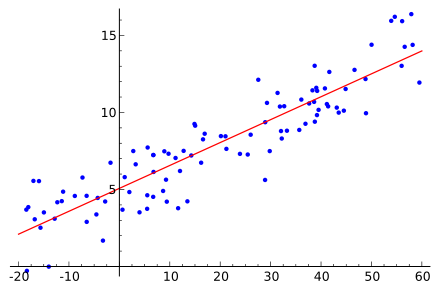
\includegraphics[scale=0.35]{imagenes/Linear_regression.png}
\end{figure}

\end{itemize}

} 
 
\end{frame}


\begin{frame}{Coeficiente de Determinación $R^2$}
\scriptsize{
\begin{itemize}
 \item Una vez ajustado nuestro modelo lineal debemos evaluar la calidad del modelo.
 \item Una medida muy común es el coeficiente de determinación $R^2$. 
 \item Para calcularlo debo calcular otros errores distintos a los errores cuadráticos SSE.
 \item Se define a la suma cuadrática total (SST) como el error predictivo cuando usamos la media $\overline{y}$ para predecir la variable de respuesta $y$ (es muy similar a la varianza de la variable):
 \begin{displaymath}
  \text{SST} = \sum_{i}^{m}(y_i-\overline{y})^2  
 \end{displaymath}
 \item Luego tenemos a la suma de los cuadrados explicada por el modelo (SSM) que nos indica la variabilidad de los valores predichos por el modelo respecto a la media:
 \begin{displaymath}
  \text{SSM} = \sum_{i}^{m}(\hat{y}_i-\overline{y})^2 
 \end{displaymath}
  
\end{itemize}

}
\end{frame}

\begin{frame}{Coeficiente de Determinación $R^2$ (2)}
\scriptsize{
\begin{itemize}
 \item Se define el coeficiente de determinación para un modelo lineal $R^2$ como:
 \begin{equation}
  R^2= \frac{\text{SSM}}{\text{SST}} = \frac{\sum_{i}^{m}(\hat{y}_i-\overline{y})^2 }{\sum_{i}^{m}(y_i-\overline{y})^2  }
 \end{equation}

 \item El coeficiente adquiere valores entre $0$ a $1$ y mientras más cercano a 1 sea su valor mayor sera la calidad del modelo.
 
 \item El valor de $R^2$ es equivalente a la correlación lineal (Pearsons) entre $y$ e $\hat{y}$ al cuadrado.
\begin{displaymath}
 R^2=\text{cor}(y,\hat{y})^2
\end{displaymath}
  
\end{itemize}


}
\end{frame}

\begin{frame}{Regresión Lineal Múltiple}
\scriptsize{
\begin{itemize}
 \item Supongamos que tenemos $n$ variables independientes: $x_1,x_2,\dots,x_n$.
 \item Intuitivamente, estas variables en conjunto podrían explicar de mejor manera la variabilidad de la variable de respuesta $\mathbf{y}$ que un modelo simple.
 \item Se define un modelo lineal multi-variado de la siguiente manera:
 \begin{displaymath}
 y_i=\beta_{0}+\beta_{1}x_{i,1}+ \beta_{2}x_{i,2} + \cdots + \beta_{n}x_{i,n} +  \epsilon_i \quad \forall i \in \{1,m\}
\end{displaymath}
\item En el modelo multi-variado se extienden todas las propiedades del modelo lineal simple.

\item Se puede representar el problema de manera matricial:
\begin{displaymath}
 Y=X\beta+\epsilon
\end{displaymath}

\item Donde $Y$ es un vector de $m\times 1$ de variables de respuesta:

\begin{displaymath}
 Y =
 \begin{pmatrix}
  y_{1} \\
  y_{2}  \\
  \vdots  \\
  y_{m}
 \end{pmatrix}
\end{displaymath}






\end{itemize}
 

}
\end{frame}

\begin{frame}{Regresión Lineal Múltiple (2)}
\scriptsize{
\begin{itemize} 
\item $X$ es una matriz de $m \times (n+1)$ con las variables explicativas. Tenemos $m$ observaciones de las $n$ variables. La primera columna es constante igual a $1$ ($x_{i,0}=1 \quad \forall i$) para modelar la variable de intercepto $\beta_0$.

\begin{displaymath}
 X =
 \begin{pmatrix}
x_{1,0} &  x_{1,1} & x_{1,2} & \cdots & x_{1,n} \\
x_{2,0} &  x_{2,1} & x_{2,2} & \cdots & x_{2,n} \\
\vdots  &  \vdots  & \vdots  & \ddots & \vdots  \\
x_{m,0} &  x_{m,1} & x_{m,2} & \cdots & x_{m,n}
 \end{pmatrix}
\end{displaymath}

 \item Luego, $\beta$ es un vector de parámetros de $(n+1) \times 1$

\begin{displaymath}
 \beta =
 \begin{pmatrix}
  \beta_{0}  \\
  \beta_{1}  \\
  \vdots    \\
  \beta_{n} 
 \end{pmatrix}
\end{displaymath}





\end{itemize}
 

}
\end{frame}

\begin{frame}{Regresión Lineal Múltiple (2)}
\scriptsize{
\begin{itemize}
\item Finalmente, $\epsilon$ es un vector con los errores del modelo de $m \times 1$. 

\begin{displaymath}
 \epsilon =
 \begin{pmatrix}
  \epsilon_{1}  \\
  \epsilon_{2}  \\
  \vdots    \\
  \epsilon_{m} 
 \end{pmatrix}
\end{displaymath}

\item Usando la notación matricial, podemos ver que la suma de los errores cuadráticos (SSE) se puede expresar como:
\begin{displaymath}
 \text{SSE} = (Y - X\beta)^{T}(Y-X\beta)
\end{displaymath}

\item Minimizando esta expresión derivando el error en función de $\beta$ e igualando a cero se llega a las ecuaciones normales:

\begin{displaymath}
   \hat{\beta} = (X^{T}X)^{-1} X^{T}Y
\end{displaymath}


\end{itemize}


}

\end{frame}

\begin{frame}{Supuestos del Modelo Lineal}
\scriptsize{





Cada vez que ajustamos un modelo lineal estamos asumiendo implícitamente ciertos supuestos sobre los datos. 


\begin{block}{Supuestos}
\begin{enumerate}
\item Linealidad: la variable de respuesta se relaciona linealmente con los atributos. 
\item Normalidad: los errores tienen distribución normal de media cero: $\epsilon_{i} \sim N(0,\sigma^2)$ 
\item Homocedasticidad: los errores tienen  varianza constante (mismo valor $\sigma^2$).
\item Independencia: los errores son independientes entre sí.
 
\end{enumerate}
 
\end{block}

} 
\end{frame}


\begin{frame}{Interpretación Probabilística}
\scriptsize{
\begin{itemize}
 \item Considerando los supuestos anteriores podemos ver que la densidad de probabilidad (PDF) de los errores $\epsilon$ esta definida por una normal de media cero y varianza constante:
 \begin{displaymath}
  \text{PDF}(\epsilon_{i})=\frac{1}{\sqrt{2\pi} \sigma} \exp \left(- \frac{\epsilon_{i}^{2}}{2\sigma^2}\right)
 \end{displaymath}
 \item Esto implica que:
  \begin{displaymath}
  \text{PDF}(y_i|x_{i};\beta)=\frac{1}{\sqrt{2\pi} \sigma} \exp \left(- \frac{(y_i - h_{\beta}(x_{i}) )^{2}}{2\sigma^2}\right)
 \end{displaymath}
 \item Lo que implica que la distribución de $\mathbf{y}$ dada los valores de $\mathbf{x}$ y parametrizada por $\beta$ sigue una distribución normal.
 \item Luego si uno estima los parámetros de $\beta$ usando una técnica de estimación llamada máxima verosimilitud llega a los mismos resultados que haciendo estimación por mínimos cuadrados.
 \item Esto nos dice que cuando estimamos los parámetros del modelo usando mínimos cuadrados estamos realizando las mismas hipótesis probabilísticas mencionados anteriormente.
 

\end{itemize}


}
 
\end{frame}

\begin{frame}[fragile]{Regresiones en R}
\scriptsize{
\begin{itemize}
 \item En R lo modelos lineales se crean con el comando \verb+lm+ que recibe como parámetro una fórmula de la forma \verb+y~x+ ($y=f(x)$).
 \item Vamos a trabajar con el dataset \verb+USArrests+ que tiene información sobre los arrestos ocurridos en Estados Unidos el año 1973. 
 \item Cada observación corresponde a un estado.
 \item Tiene las siguientes variables:
 \begin{enumerate}
 \scriptsize{
  \item \textbf{Murder}:  arrestos por homicidio (por 100.000 habitantes).
  \item \textbf{Assault} : arrestos por asalto (por 100.000 habitantes).
  \item \textbf{UrbanPop}: porcentaje de la población total del estado.
  \item \textbf{Rape}: arrestos por violación (por 100.000 habitantes).
  }
 \end{enumerate}
 
\item Para ver si vale la pena hacer un análisis de regresión lineal vemos las correlaciones lineales entre las variables: 

 \begin{verbatim}
> data(USArrests)
> attach(USArrests)
> cor(USArrests)
             Murder   Assault   UrbanPop      Rape
Murder   1.00000000 0.8018733 0.06957262 0.5635788
Assault  0.80187331 1.0000000 0.25887170 0.6652412
UrbanPop 0.06957262 0.2588717 1.00000000 0.4113412
Rape     0.56357883 0.6652412 0.41134124 1.0000000  
 \end{verbatim}

 
 
 
\end{itemize}
 
 
 
 
} 
\end{frame}

\begin{frame}[fragile]{Regresiones en R (2)}
\scriptsize{
\begin{itemize}
 \item Podemos ver que hay una correlación positiva importante entre \verb+Murder+ y \verb+Assault+.
 \item Vamos a modelar los asesinatos en función de los asaltos usando una regresión lineal simple:
 \begin{displaymath}
  \text{Murder}(\text{Assault})=\beta_0+\beta_1*\text{Assault}
 \end{displaymath}
 \begin{verbatim}
> reg1<-lm(Murder~Assault,USArrests)
> reg1

Call:
lm(formula = Murder ~ Assault, data = USArrests)

Coefficients:
(Intercept)      Assault  
    0.63168      0.04191    
 \end{verbatim}
 
 \item Podemos ver que los coeficientes del modelo son $\beta_{0}=0.632$ y $\beta_{1}=0.042$. 
 
 


\end{itemize}
 
 
 
} 
\end{frame}

\begin{frame}[fragile]{Regresiones en R (3)}
\scriptsize{
\begin{itemize}
 \item Podemos acceder directamente a los coeficientes y guardarlos en una variable:
 \begin{verbatim}
> reg1.coef<-reg1$coefficients
> reg1.coef
(Intercept)     Assault 
 0.63168266  0.04190863 
 \end{verbatim}
 
\item Podemos ver diversos indicadores sobre el modelo lineal con el comando \textbf{summary}:
 
\begin{verbatim}
> summary(reg1)
Residuals:
    Min      1Q  Median      3Q     Max 
-4.8528 -1.7456 -0.3979  1.3044  7.9256 

Coefficients:
            Estimate Std. Error t value Pr(>|t|)    
(Intercept) 0.631683   0.854776   0.739    0.464    
Assault     0.041909   0.004507   9.298  2.6e-12 ***
---
Signif. codes:  0 ‘***’ 0.001 ‘**’ 0.01 ‘*’ 0.05 ‘.’ 0.1 ‘ ’ 1

Residual standard error: 2.629 on 48 degrees of freedom
Multiple R-squared:  0.643,	Adjusted R-squared:  0.6356 
F-statistic: 86.45 on 1 and 48 DF,  p-value: 2.596e-12

\end{verbatim}
 
 \end{itemize}
 
 


} 
\end{frame}


\begin{frame}[fragile]{Regresiones en R (4)}
\scriptsize{
\begin{itemize}
 \item Vemos que el coeficiente de determinación $R^2$ tiene un valor de $0.643$ lo cual no es tan bueno pero aceptable.
 
 
  \item Podemos concluir que el nivel de asaltos si bien provee información útil para modelar una parte de la variabilidad del nivel de homicidios no es suficiente para construir un modelo altamente confiable. 
  
  \item Puedo guardar los resultados del comando \verb+summary+ en una variable y así acceder directamente al coeficiente de determinación:
\begin{verbatim}
> sum.reg1<-summary(reg1)
> sum.reg1$r.squared
[1] 0.6430008   
\end{verbatim}

\item También puedo acceder a los valores ajustados que son los valores predichos por mi modelo para los datos usados:
\begin{verbatim}
> reg1$fitted.values
       Alabama         Alaska        Arizona       Arkansas        
     10.522119      11.653652      12.952819       8.594322      
\end{verbatim}
 
 \end{itemize}
 

} 
\end{frame}



\begin{frame}[fragile]{Regresiones en R (5)}
\scriptsize{
\begin{itemize}
 \item Podemos ver que la correlación lineal al cuadrado entre mis valores ajustados y los observados para la variable de respuesta es equivalente al coeficiente de determinación:
 
 \begin{verbatim}
> cor(Murder,reg1$fitted.values)^2
[1] 0.6430008
 \end{verbatim}

\item Supongamos ahora que conozco el nivel de asalto de dos estados en otro período para dos lugares pero no conozco el nivel de homicidios.

\item Podría usar mi modelo lineal para predecir el nivel de de homicidios.

\item Para hacerlo en R debo usar el comando \verb+predict.lm+ que recibe el modelo lineal y un data.frame con los datos nuevos:
\begin{verbatim}
> nuevos.arrestos<-data.frame(Assault=c(500,12))
> predict.lm(object=reg1,newdata=nuevos.arrestos)
        1         2 
21.585997  1.134586 
> # Esto es equivalente a:
> reg1.coef[1]+reg1.coef[2]*nuevos.arrestos
    Assault
1 21.585997
2  1.134586 
\end{verbatim}

 
 \end{itemize}
 

} 
\end{frame}


\begin{frame}[fragile]{Regresiones en R (6)}
\scriptsize{
\begin{itemize}
 \item Ahora estudiaremos una regresión lineal múltiple.
 \item Podemos ver que la variable \textbf{Rape} que representa el nivel de violaciones tiene una correlación menor con el número de asaltos y con el número de homicidios que la correlación que presentan estas dos variables entre sí.
 \item Vamos a ajustar el siguiente modelo lineal multi-variado:
 \begin{displaymath}
 \text{Rape}=\beta_{0}+\beta_{1}*\text{Assault}+\beta_{2}*\text{Murder}
 \end{displaymath}
 \item En R para agregar más variables al modelo lineal las agregamos con el signo \textbf{+} :
\begin{verbatim}
reg2<-lm(Rape~Assault+Murder,USArrests)
\end{verbatim}



 
 \end{itemize}
 

} 
\end{frame}


\begin{frame}[fragile]{Regresiones en R (7)}
\scriptsize{

\begin{verbatim}
> summary(reg2)

Residuals:
    Min      1Q  Median      3Q     Max 
-17.243  -3.171  -1.171   3.281  18.511 

Coefficients:
            Estimate Std. Error t value Pr(>|t|)    
(Intercept)  8.35011    2.32912   3.585 0.000799 ***
Assault      0.06716    0.02044   3.286 0.001927 ** 
Murder       0.18155    0.39108   0.464 0.644619    
---
Signif. codes:  0 ‘***’ 0.001 ‘**’ 0.01 ‘*’ 0.05 ‘.’ 0.1 ‘ ’ 1

Residual standard error: 7.124 on 47 degrees of freedom
Multiple R-squared:  0.4451,	Adjusted R-squared:  0.4215 
F-statistic: 18.85 on 2 and 47 DF,  p-value: 9.755e-07

\end{verbatim}

\begin{itemize}
\item En este caso el coeficiente de determinación es bajo. Por lo que tendremos baja confianza en la calidad del modelo.
 \end{itemize}
 

} 
\end{frame}

\begin{frame}[fragile]{Regresiones en R (8)}
\scriptsize{
\begin{itemize}
 \item Cuando teníamos una regresión simple podíamos ver el modelo ajustado como una recta.
 \item Ahora que tenemos dos variables independientes podemos ver el modelo ajustado como un plano.
 \item Si tuviésemos más variables independientes nuestro modelo sería un hiper-plano.
 \item Podemos graficar en R el plano de nuestro modelo lineal de dos variables independientes y una dependiente de la siguiente manera:
 \end{itemize}

\begin{verbatim}
library("scatterplot3d")
s3d <- scatterplot3d(USArrests[,c("Assault","Murder","Rape")],
                     type="h", highlight.3d=TRUE,
                     angle=55, scale.y=0.7, pch=16, 
                     main="Rape~Murder+Rape")
s3d$plane3d(reg2, lty.box = "solid")

\end{verbatim}




} 
\end{frame}

\begin{frame}{Regresiones Lineales en R (9)}
 
\begin{figure}[h!]
	\centering
	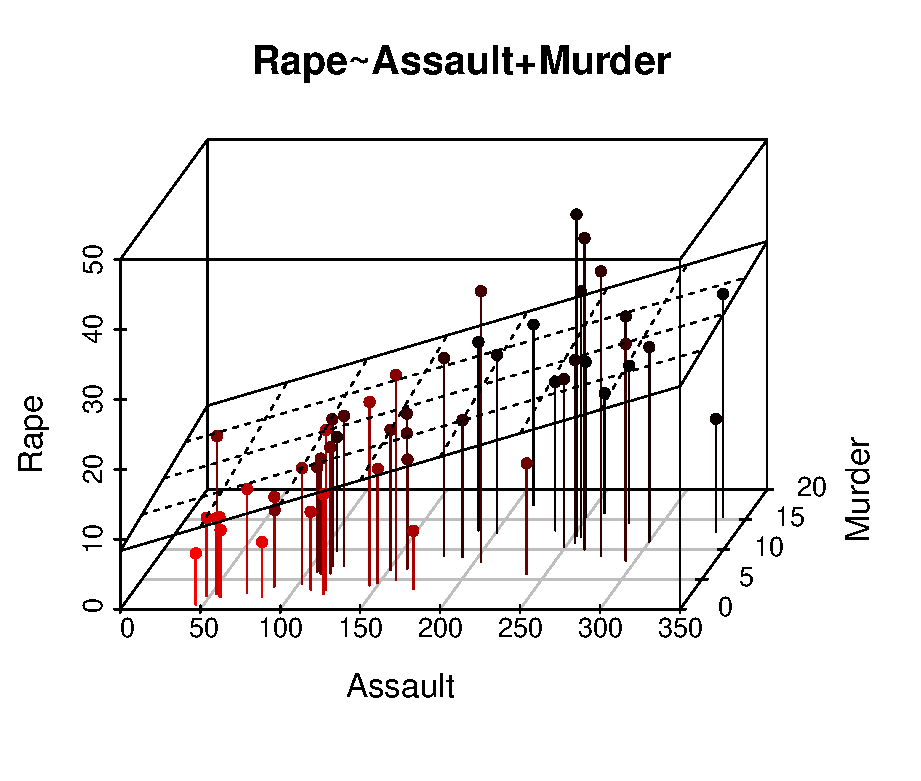
\includegraphics[scale=0.6]{imagenes/reg3d.pdf}
\end{figure}
 
\end{frame}


\begin{frame}{Entrenando un modelo lineal}
\begin{scriptsize}
\begin{itemize}
\item Una forma alternativa a ver el problema de regresión es definiendo una  función de pérdida $L(\hat {y}, y)$, indicando la pérdida o error de la predicción de $\hat{y}$ cuando la salida verdadera es y.

\item Una función de pérdida calcula un escalar a partir de $\hat{y}$ e $y$. 

\item Una función de pérdida a usar  para regressión es el error cuadrático medio (MSE), que es el SSE normalizado por la cantidad de ejemplos.

\begin{equation}
MSE = \frac{1}{m}\sum_{i=1}^{m} (y_i-h(x_i))^2 
\end{equation}

\item El objetivo del entrenamiento es minimizar la pérdida en los datos de entrenamiento.


\end{itemize}


\end{scriptsize}
\end{frame}


\begin{frame}{Entrenando un modelo lineal}
\begin{scriptsize}
\begin{itemize}

\item La regresión lineal es un caso particular de modelo de regresión donde los parámetros tienen solución exacta (ecuaciones normales).

\item Alternativamente, una regresión se puede se entrenar usando métodos iterativos basados en gradientes.


\item Se calculan los gradientes de los parámetros con respecto a la pérdida $L$, y se mueven los parámetros en las direcciones opuestas del gradiente.


\item Diferentes métodos de optimización difieren en cómo se calcula la estimación del error y cómo se define el movimiento en la dirección opuesta al gradiente.

\end{itemize}


\end{scriptsize}
\end{frame}


\begin{frame}{Descenso del Gradiente}
\begin{figure}[htb]
	\centering
	 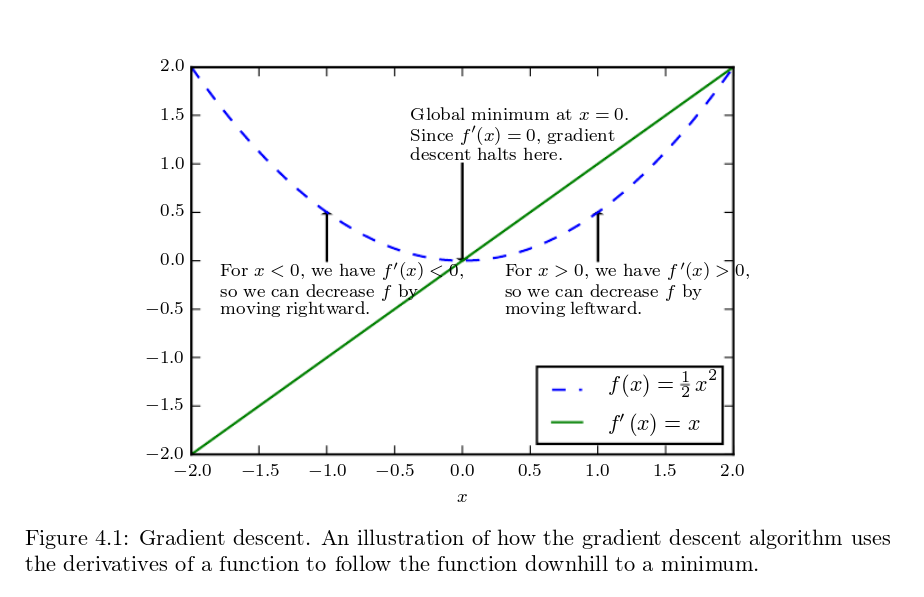
\includegraphics[scale=0.45]{imagenes/gradientdescent.png}
\end{figure}

\footnotetext{\cite{deepbook}}

\end{frame}


\begin{frame}{Descenso del Gradiente}
\begin{figure}[htb]
	\centering
	 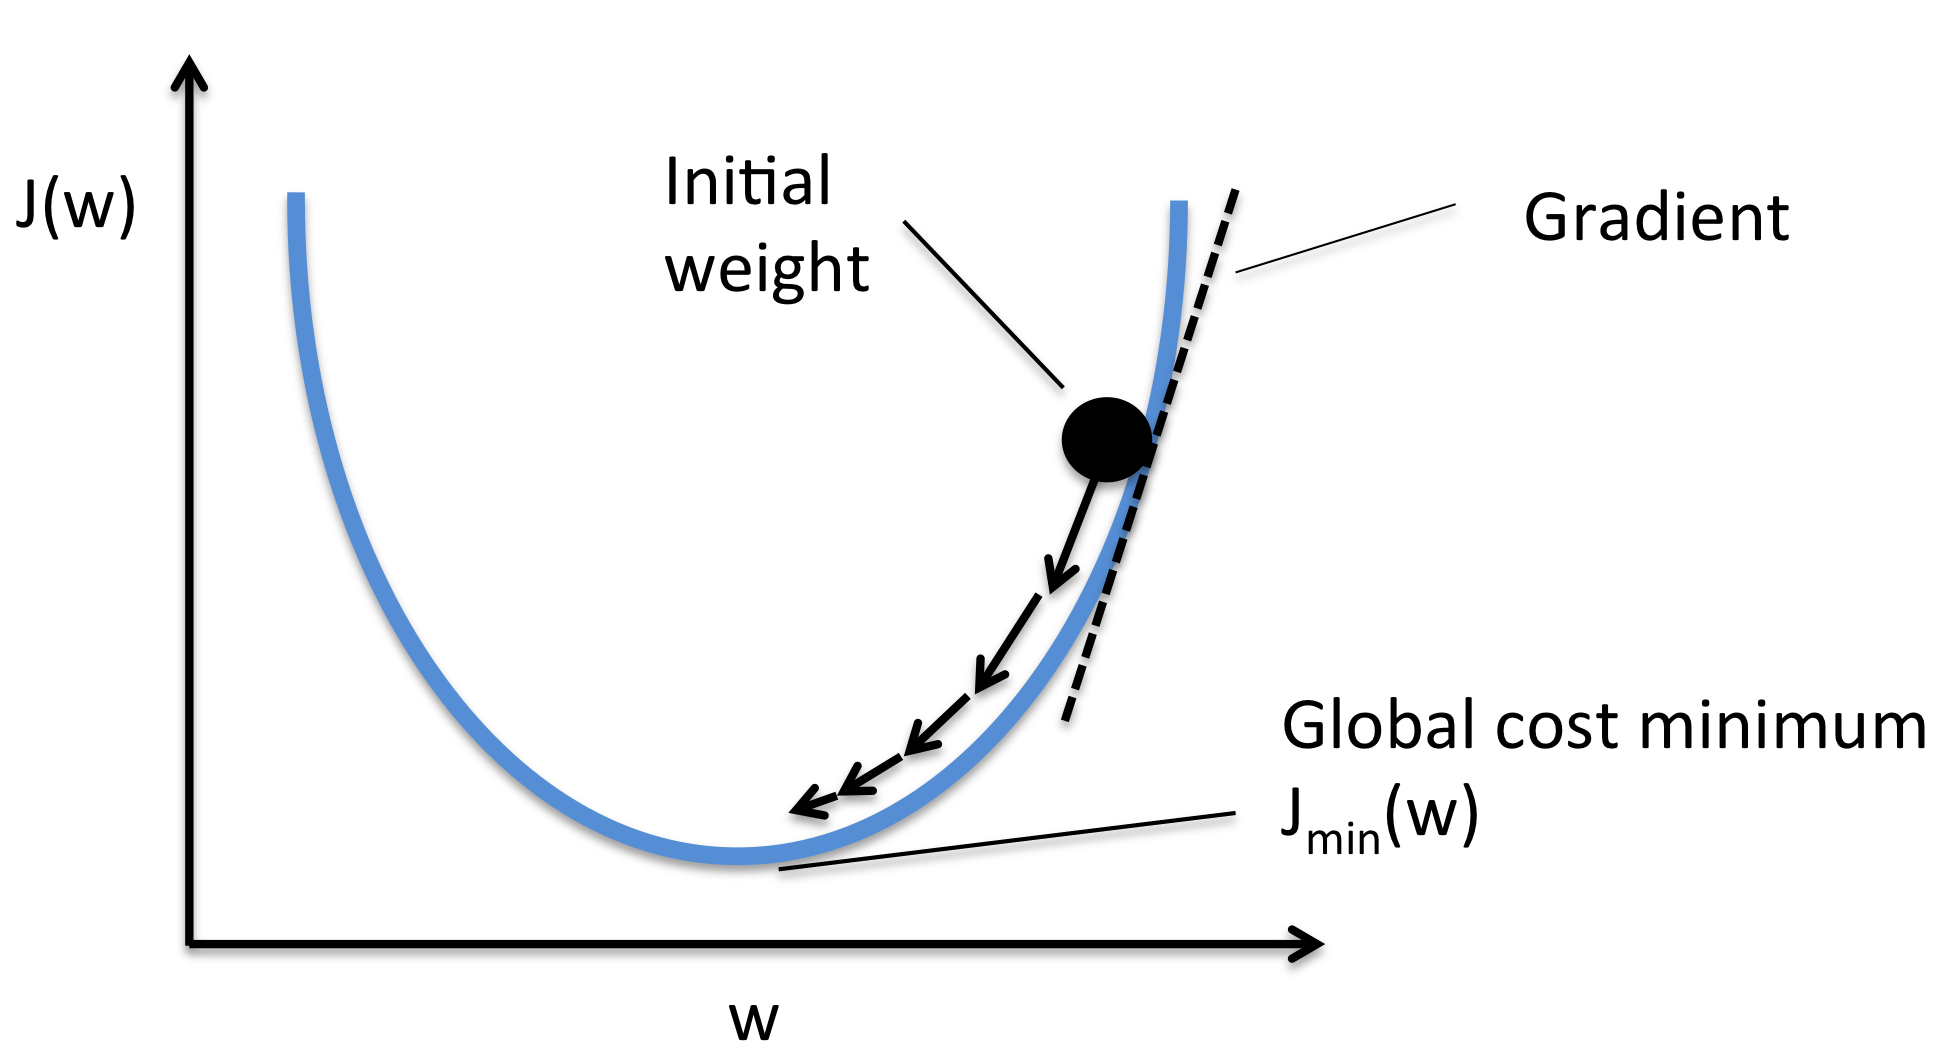
\includegraphics[scale=0.15]{imagenes/sgd.png}
\end{figure}

\footnotetext{Source: \url{https://sebastianraschka.com/images/faq/closed-form-vs-gd/ball.png}}


\end{frame}

\begin{frame}{Descenso del Gradiente}
\begin{figure}[htb]
	\centering
	 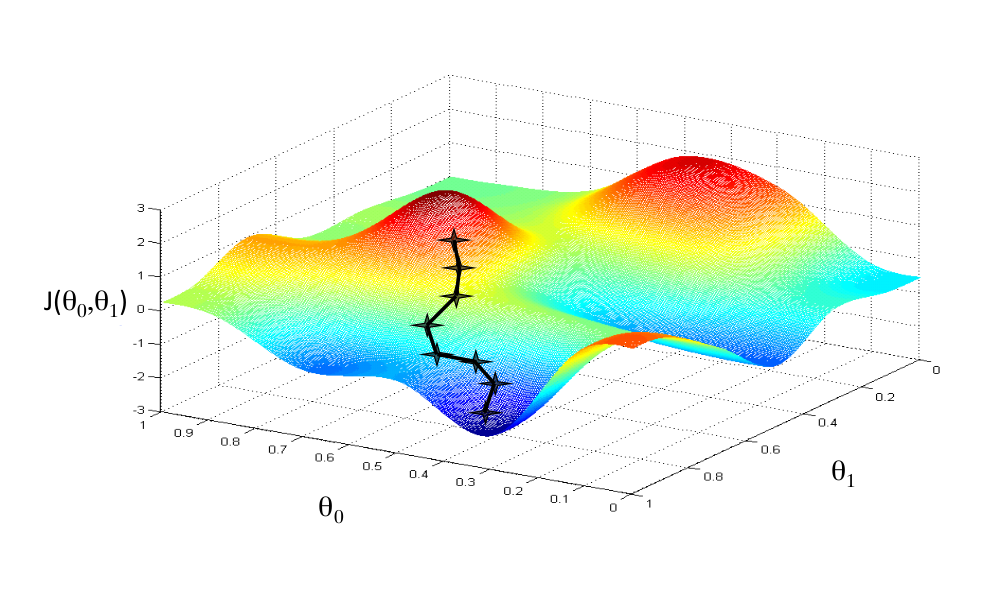
\includegraphics[scale=0.4]{imagenes/gradientdescent2.png}
\end{figure}



\end{frame}






\begin{frame}{Descenso del Gradiente Online Estocástico (SGD)}

\begin{scriptsize}
\begin{itemize}
\item Se inicializan los parámetros $w$ con valores iniciales aleatorios.
\item Por cada dato de entramiento $(x,y)$ calculo $L$ con el valor actual de $w$ y actualizo los parámetros usando la siguiente regla hasta converger:
\item $w_i \leftarrow w_i - \eta \frac{\partial L}{w_i}(x,y)$  (Para todos los parámetros $w_i$)

\begin{figure}[htb]
	\centering
	 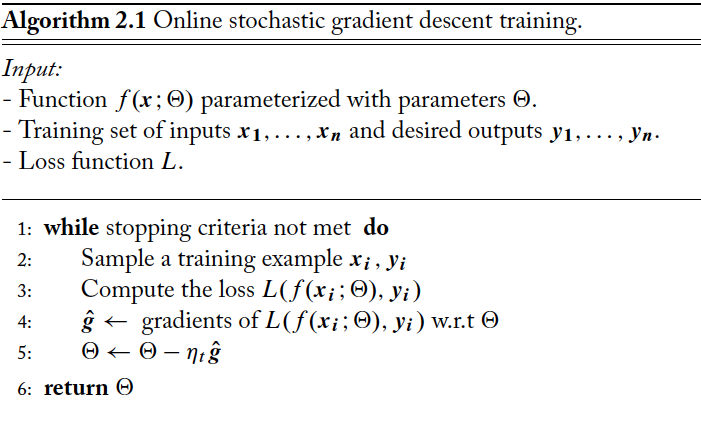
\includegraphics[scale=0.3]{imagenes/Online-SGD.png}
\end{figure}

\end{itemize}


\end{scriptsize}


\end{frame}

\begin{frame}{Descenso del Gradiente Online Estocástico (SGD)}

\begin{scriptsize}
\begin{itemize}

\item La tasa de aprendizaje $\eta$ puede ser fija a lo largo del proceso de entrenamiento, o se puede decaer en función del paso de tiempo $t$.
\item El error calculado en la línea 3 se basa en un solo dato de entrenamiento  y, por lo tanto, es solo una estimación aproximada de la pérdida total $L$ que queremos minimizar.
\item El ruido en el cálculo de la pérdida puede dar lugar a gradientes inexactos (un solo dato puede proporcionar información ruidosa).
\end{itemize}


\end{scriptsize}


\end{frame}


\begin{frame}{Funciones de Pérdida para clasificación}
\begin{scriptsize}
El MSE es una función de pérdida para entrenar modelos de regresión. También se puede tener funciones de pérdida para entrenar modelos de clasificación:
\begin{itemize}
 \item Hinge (función bisagra): para problemas de clasificación binaria, la salida del clasificador es un escalar $\tilde{y}$ y la salida deseada $y$ está en $\{+1,-1\}$.  La regla de clasificación es $\hat{y} = sign(\tilde{y})$, y la clasificación se considera correcta cuando $y \cdot \tilde{y} > 0$.  
 \begin{displaymath}
  L_{\text{hinge}(\text{binary})}(\tilde{y},y) = \max(0,1-y \cdot \tilde{y})  
 \end{displaymath}
 
 \item Esta es la función de pérdida de la SVM (hiperplano de máximo margen). 
 
 \item ¡Podemos entrenar una SVM lineal usando SGD!
 
 \item ¿Es $\max$ una función derivable? Para aplicar SGD a $\max(0,x)$, el valor del gradiente es 1 cuando $x>0$ y 0 para el caso contrario.

 
\end{itemize}
\end{scriptsize}

\end{frame}



\begin{frame}{Regresión Logística}
\begin{scriptsize}
\begin{itemize}
\item Una regresión logística estima la probabiliad posterior  $P(y|x)$ de una variable binaria $y$ dado los datos obervados $x$ ajustando un modelo lineal a los datos.

\item Los parámetros del modelo son un vector de parámetros $w$.

\item Si asumimos el término de intercepto como 1 $x_0=1$, tenemos una función lineal de la siguiente forma:


\begin{equation}
 \tilde{y}=\sum_{i=0}^{n}w_{i}x_{i}=w^Tx
\end{equation}

\item Para darle una interpretación probabilística a la salida, transformamos $\tilde{y}$ al intervalo $[0,1]$ usando una función sigmoidal.:

\begin{equation}
g(z)=\frac{1}{1+e^{-z}}
\end{equation}
 
 
\end{itemize}
\end{scriptsize}

\end{frame}

\begin{frame}{Regresión Logística}

\begin{figure}[htb]
	\centering
	 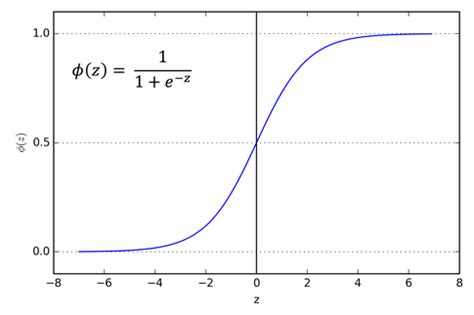
\includegraphics[scale=0.35]{imagenes/sigmoid.jpeg}
\end{figure}



\begin{scriptsize}
\begin{itemize}
\item Esto se puede resumir en la  función de perdida logística:

  \begin{displaymath}
  L_{\text{logistic}}(\hat{y},y) = -y \log \hat{y} - (1-y) \log(1-\hat{y})  
 \end{displaymath}


 \item Esta función de perdida es entonces el negativo del log-likelihood de un modelo probabilístico donde $P(y|x)$ sigue una distribución de Bernoulli.

 \item Muchas funciones de perdidas son el negativo de una función de verosimilitud. Entonces, minimizar la pérdida equivale en esos casos a realizar estimación por máxima verosimilitud. 
 
 \item ¡Podemos entrenar una regresión logística usando SGD!
 
\end{itemize}
\end{scriptsize}

\end{frame}


%\begin{frame}{ Categorical cross-entropy}
%\begin{scriptsize}
%\begin{itemize}
%
% \item Categorical cross-entropy loss:  se usa para tener una interpretación probabilística a un problema de clasificación de múltiples clases. Mide la disimilitud entre la distribución real de las clases $y$ y la distribución predicha $\tilde{y}$. 
%   \begin{displaymath}
%  L_{\text{cross-entropy}}(\hat{y},y) = - \sum_{i} y_{[i]} \log(\hat{y}_{[i]})   
% \end{displaymath}
%\item Para la cross-entropy loss ($\hat{y}$) primero hay que transformar la salida del modelo lineal $\tilde{y}$ usando una función softmax:
%    \begin{displaymath}
%\hat{y}_{[i]} = \text{softmax}(\tilde{y})_{[i]} =  \frac{e^{\tilde{y}_{[i]}}}{\sum_{j}e^{\tilde{y}_{[j]}}}   
% \end{displaymath}
 
%\item La función softmax transforma la salida de $k$ dimensiones a valores en el rango (0,1) con todos los valores sumando 1. Por lo tanto, $\hat{y}_{[i]} = P (y = i | x) $ representa la distribución condicional de los miembros de la clase.
 
%\end{itemize}
%\end{scriptsize}


%\end{frame}



\begin{frame}{Introducción a las redes neuronales}
\begin{scriptsize}
\begin{itemize}
\item Una gran limitación de los modelos lineales que sólo pueden encontrar relaciones lineales entre la entrada y la salida.
\item Las redes neuronales son modelos de aprendizaje automático muy populares formados por unidades llamadas \textbf{neuronas}.
\item Son capaces de aprender relaciones no-lineales entre $x$ e $y$.
\item También se pueden entrenar con métodos de gradiente.
\end{itemize}


\end{scriptsize}
\end{frame}



\begin{frame}{Introducción a las redes neuronales}
\begin{scriptsize}
\begin{itemize}
\item Una neurona es una unidad computacional que tiene entradas y salidas escalares.
\item Cada entrada tiene un peso asociado $w$.
\item La neurona multiplica cada entrada por su peso y luego las suma (también se pueden usar otras funciones de agreación como \textbf{max}).
\item Aplica una función de activación $g$ (generalmente no lineal) al resultado, y la pasa a su salida.
\item Se pueden apilar varias capas.
\item A este tipo de redes se les conoce como Feedforward Networks o Multi-Layer Perceptron.
\end{itemize}


\end{scriptsize}
\end{frame}


\begin{frame}{Feedforward Network de dos capas}


\begin{figure}[htb]
	\centering
	 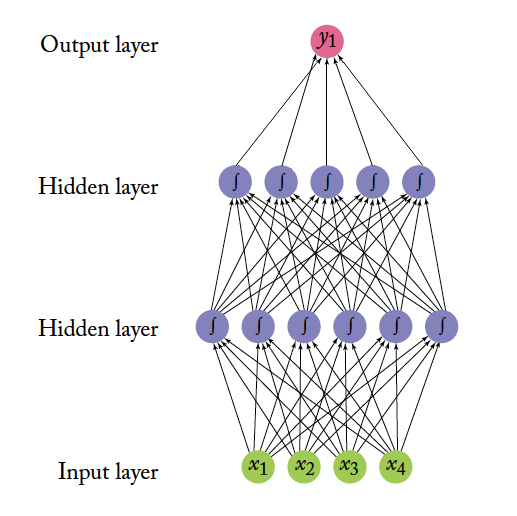
\includegraphics[scale=0.38]{imagenes/NN-example.png}
\end{figure}

\footnotetext{Source:\cite{goldberg2016primer}}

\end{frame}



\begin{frame}{Funciones de activación}

\begin{scriptsize}
\begin{itemize}
\item La función de activación no lineal $g$ tiene un papel crucial en la capacidad de la red para representar funciones complejas.
\item Si quitamos la no-linealidad aportada por $g$, la red neuronal sólo podría representar transformaciones lineales de la entrada.

\end{itemize}


\end{scriptsize}

\begin{figure}[htb]
	\centering
	 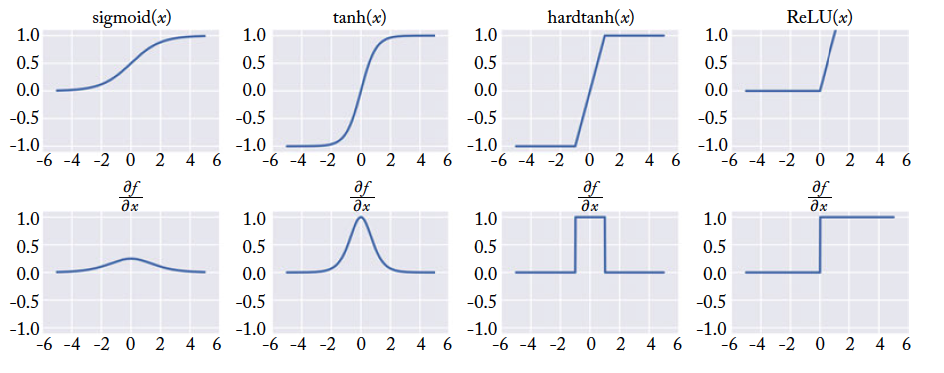
\includegraphics[scale=0.3]{imagenes/activations.png}
\end{figure}

\footnotetext{Source:\cite{goldberg2016primer}}

\end{frame}





\begin{frame}{Redes Feedforward}
\begin{scriptsize}
\begin{itemize}
\item La red feedforward de la imagen es una pila de modelos lineales separados por funciones no lineales.
\item Los valores de cada fila de neuronas en la red se pueden considerar como un vector. 

\item La capa de entrada es un vector de 4 dimensiones $(\vec{x})$, y la capa de arriba es un vector de 6 dimensiones $(\vec{h}^1)$.


\item Esta capa de conexión completa se puede ver una transformación lineal de 4 a 6 dimensiones.
\item Una capa de conexión completa implementa una multriplicación vector-matriz, $\vec{h}=\vec{x}W$.
\item El peso de la conexión desde la neurona $i$ en la fila de entrada hasta la neurona $j$ en la fila de salida es $W_{[i, j]}$.
\item Los valores de $\vec{h}$ se transforman usando una función no lineal $g$ que se aplica a cada elemento antes de pasar como entrada a la siguiente capa.
\end{itemize}


\footnotetext{En la notación asumimos que los vectores son filas y los superíndices corresponden a capas de red.}

\end{scriptsize}
\end{frame}


\begin{frame}{Capa complementamente conectado como una multiplicación vector por matriz}
\begin{figure}[htb]
	\centering
	 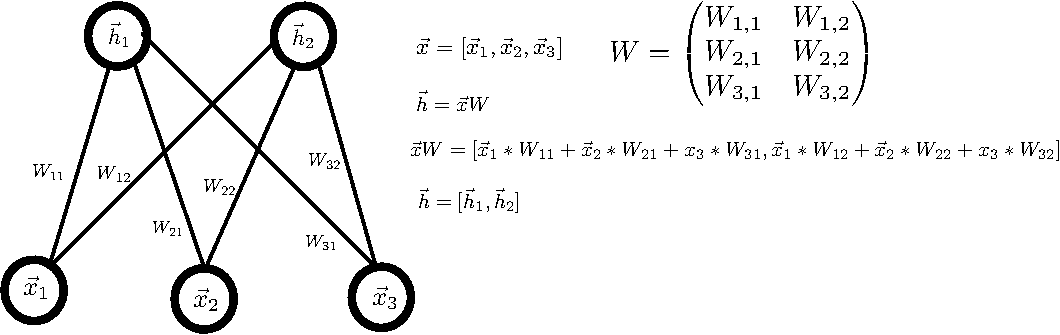
\includegraphics[scale=0.65]{imagenes/neural_net_mat_mul.pdf}
\end{figure}
\end{frame}


\begin{frame}{La red como una función}
\begin{scriptsize}
\begin{itemize}
\item El perceptrón multicapa (MLP) de la figura se puede escribir como la siguiente función matemática:
\begin{center}
\begin{equation}
\begin{split}
NN_{MLP2}(\vec{x}) & =  \vec{y}  \\
\vec{h}^{1} &  = g^{1}(\vec{x}W^{1}+\vec{b}^{1}) \\
\vec{h}^{2} &  = g^{2}(\vec{h}^{1}W^{2}+\vec{b}^{2}) \\
\vec{y} &  = \vec{h}^{2}W^{3}\\
\vec{y} &  = (g^2(g^1(\vec{x}W^{1}+\vec{b}^{1})W^2+\vec{b}^2))W^3.\\
\end{split}
\end{equation}
\end{center}
%NN_{MLP2(x)}  =  y \\
%h^{1} = g^{1}(xW^{1}+b{1}) \\

\end{itemize}


\end{scriptsize}
\end{frame}







\begin{frame}{El Grafo de Cómputo}
\begin{scriptsize}
\begin{itemize}
\item Las redes neuronales se entrenan usando descenso por gradiente. 
\item En teoría, se podrían calcular los gradientes de los diversos parámetros de una red a mano e implementarlos en código.

\item Este procedimiento es engorroso y propenso a errores.

\item Es preferible usar herramientas de derivación automática [Bengio, 2012].

\item Un grafo de cómputo (computation graph) es un grafo capaz de representar cualquier proceso de cómputo matemático (e.g., evaluar una red neuronal).

\item Considere, por ejemplo el grafo computacional para $(a*b+1)*(a*b+2)$:

\begin{figure}[htb]
	\centering
	 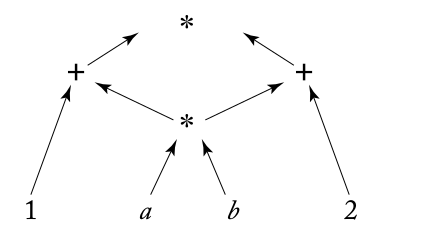
\includegraphics[scale=0.25]{imagenes/compGraph.png}
\end{figure}

\item El cálculo de $a*b$ es compartido.

\item La estructura del grafo define el orden del cálculo en términos de las dependencias entre los diferentes componentes.

\end{itemize}
\end{scriptsize}
\end{frame}






\begin{frame}{El Grafo de Cómputo}
\begin{scriptsize}
\begin{itemize}

\item  El grafo de cómputo nos permite:


\begin{enumerate}
\begin{scriptsize}
 \item Constuir fácilmente redes neuronales arbitrarias.
 \item Evaluar sus prediciones para una entrada dada (forward pass).
 
 \begin{figure}[htb]
	\centering
	 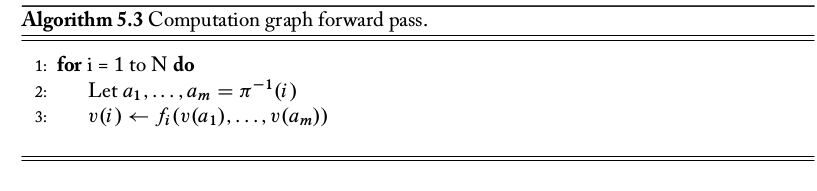
\includegraphics[scale=0.25]{imagenes/forwardPass.png}
\end{figure}

 
 
 \item  Calcular los gradientes para sus parámetros con respecto a funciones de perdida arbitrarias (backward pass o backpropagation).

 
  
 \begin{figure}[htb]
	\centering
	 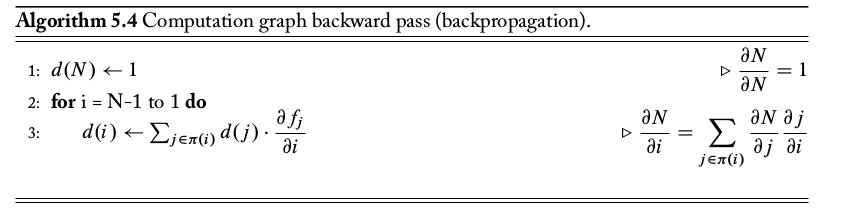
\includegraphics[scale=0.25]{imagenes/backwardPass.png}
\end{figure}
 
\end{scriptsize}
 \end{enumerate}
  
  
  
  
 \item El algoritmo de backpropagation (backward pass) escencialmente sigue la regla de la cadena en derivación\footnote{Un muy buen tutorial del algoritmo backpropagation usando la abstracción del grafo de cómputo: \url{https://colah.github.io/posts/2015-08-Backprop/}}.
 
  
\end{itemize}
\end{scriptsize}
\end{frame}


\begin{frame}{SGD por Mini-batches}


\begin{scriptsize}
\begin{itemize}
\item SGD es susceptible al ruido inducido por un único ejemplo (un outlier puede mover mucho el gradiente).
\item Una forma común para reducir este ruido es estimar el error y los gradientes sobre muestras de  $m$ ejemplos.
\item Esto se llama minibatch SGD.


\item Valores grandes para m $m$ dan una mejor estimación del gradiente en base al dataset completo, mientras que valores más pequeños permiten realizar más actualizaciones y converger más rápido.

\item Para tamaños razonables de $m$ , algunas arquitecturas computacionales (i.e., GPUs, TPUs) permiten paralelizar SGD eficientemente (es la única forma de entrenar redes de varias capas en tiempo razonable).

\end{itemize}
\end{scriptsize}


\end{frame}


\begin{frame}{Descenso de Gradiente Estocástico por Mini-batches}






\begin{figure}[htb]
	\centering
	 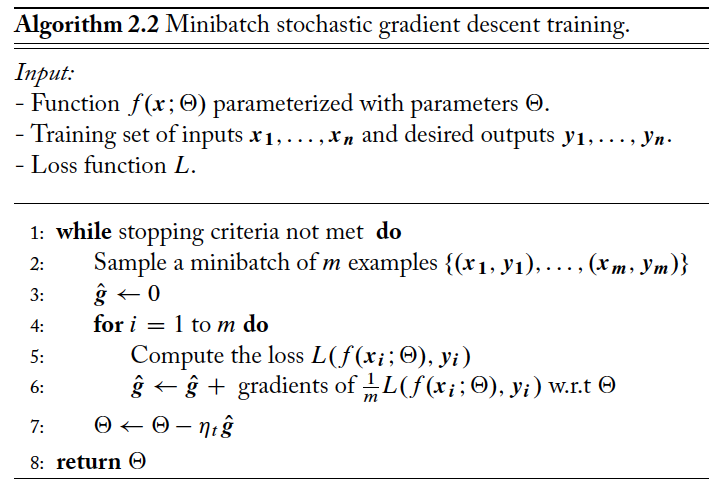
\includegraphics[scale=0.4]{imagenes/minibatch-SGD.png}
\end{figure}

\footnotetext{Source:\cite{goldberg2016primer}}

\end{frame}



\begin{frame}{Comentarios}
\begin{scriptsize}
\begin{itemize}
\item Las redes neuronales son modelos muy poderosos para regresión y clasificación. 

\item El uso de redes con varias capas se llama popularmente como Deep Learning.

\item Existen arquitecturas de red que son buenas para aprender representaciones sobre datos complejos: texto, imágenes, audio, video.

\item Arquitecturas famosas: redes neuronales convolucionales, redes recurrentes y redes de atención.

\item La alta capacidad de estas redes las hace muy proclives al overfitting.

\item Hay varias técnicas para mitigarlo: regularización, drop-out, batch normalization.


\end{itemize}
\end{scriptsize}
\end{frame}


\begin{frame}{Frameworks para Deep Learning}
Varios paquetes de software implementan el modelo de grafo de cómputo. 

Estos paquetes implementan los componentes esenciales (tipos de nodo) para definir una amplia gama de arquitecturas de redes neuronales.
\begin{scriptsize}
\begin{itemize}
\item TensorFlow (\url{https://www.tensorflow.org/}): una biblioteca de software de código abierto para cálculos numéricos utilizando data-flow graphs desarrollados originalmente por Google Brain Team.

\item Keras: API de redes neuronales de alto nivel que corre sobre Tensorflow y otros  backends (\url{https://keras.io/}). 

\item PyTorch:  biblioteca de código abierto de aprendizaje automático para Python, basada en Torch, desarrollada por el grupo de investigación de inteligencia artificial de Facebook. Es compatible con la construcción de grafos de cómputo dinámicos, se crea un gráfo de cómputo diferente desde cero para cada muestra de entrenamiento.  (\url{https://pytorch.org/})
\end{itemize}
\end{scriptsize}
\end{frame}



\begin{frame}[allowframebreaks]\scriptsize
\frametitle{Bilbiografía}
\begin{thebibliography}{8}

\bibitem{Assaad2008}
L. Wasserman \emph{All of Statistics: A Concise Course in Statistical Inference}, Springer Texts in Statistics, 2005.

\bibitem[Goldberg, 2016]{goldberg2016primer}
Goldberg, Y. (2016).
\newblock A primer on neural network models for natural language processing.
\newblock {\em J. Artif. Intell. Res.(JAIR)}, 57:345--420.

\bibitem[Goodfellow16]{deepbook}
Goodfellow, Ian, Yoshua Bengio, and Aaron Courville.
\newblock Deep learning. MIT press, 2016.



\end{thebibliography}


\end{frame}




%%%%%%%%%%%%%%%%%%%%%%%%%%%

\end{document}
